\section{Numerical experiments}
\label{s:numerics}

\subsection{$\SOn{2}$ reduced \twoMode\ system}

\begin{figure}%[H]
\centering
 (a) 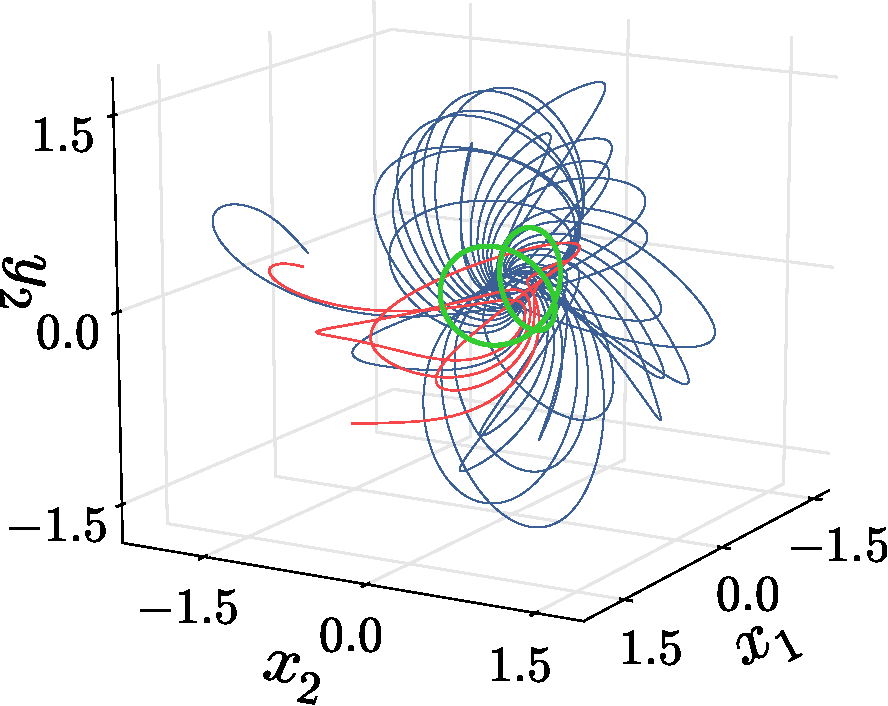
\includegraphics[width=0.20\textwidth]{2modes-ssp}
 (b) 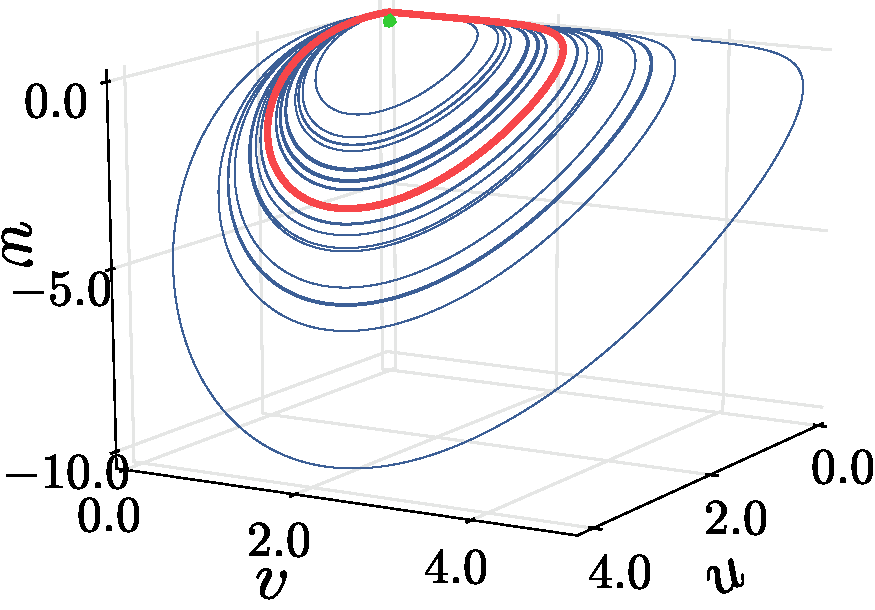
\includegraphics[width=0.20\textwidth]{2modes-invpol}
 \\
 (c) 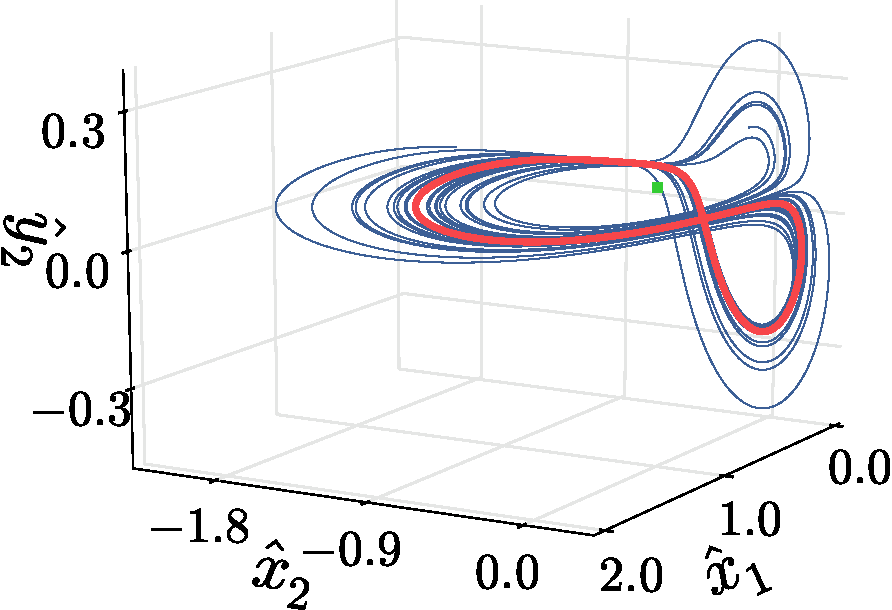
\includegraphics[width=0.20\textwidth]{2modes-sspRed}
%  (d) 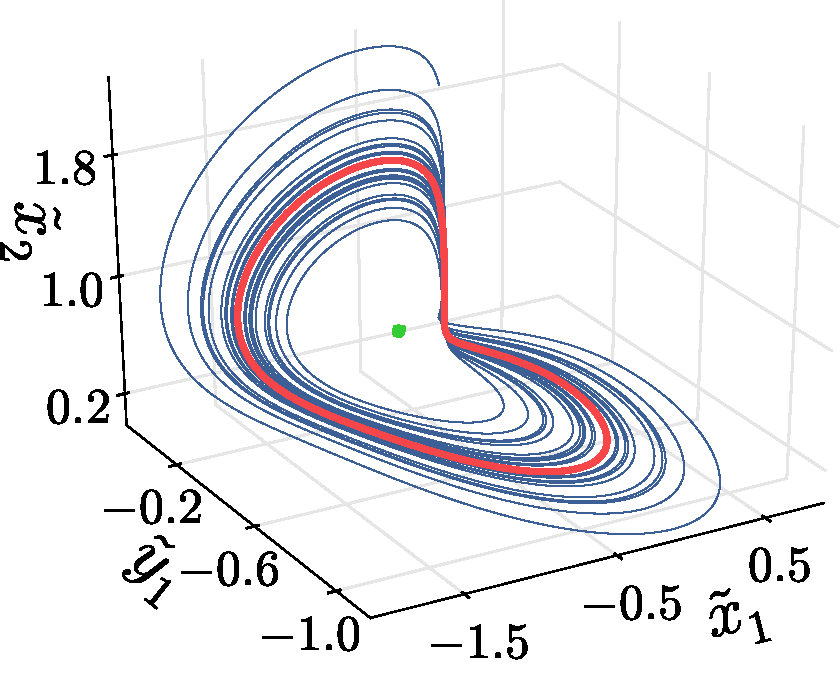
\includegraphics[width=0.20\textwidth]{2modes-sspRed2}
 (d) 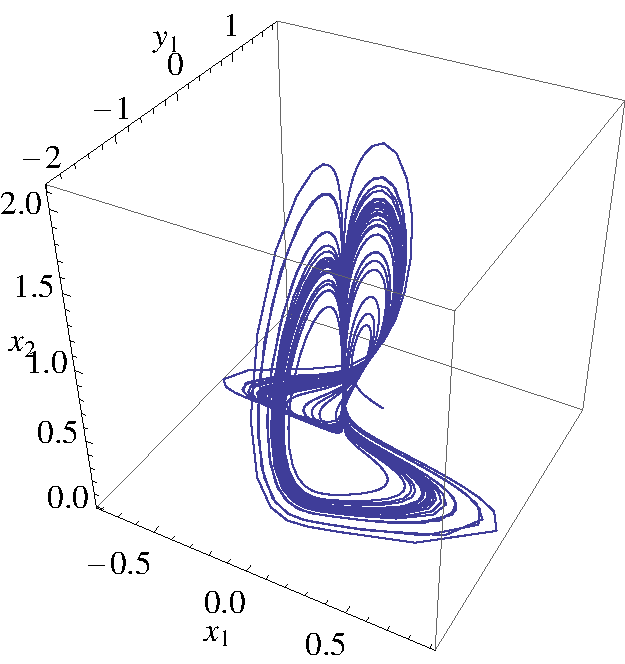
\includegraphics[width=0.20\textwidth]{2modesSliceIntFM2}
\caption{(Color online) The \twomode\ system:
A typical chaotic trajectory (blue), a trajectory spiraling out
from the \reqv\ (green), 10 repeats of the shortest
$\period{} = 3.6415120$ \rpo\
(orange) plotted in (a) a 3D projection of its
four-dimensional \statesp; (b) invariant polynomials (c) first-mode
 \slicePlane , (d) second-mode \slicePlane.}
\label{fig:Set1}
\end{figure}
\ES{2014-05-15}{I have replaced the second-mode slice, double-angled figure in \reffig{fig:Set1}(b)
with one resulting by integrating on the $(0,0,1,0)$ slice, for consistency with
panel (c). I hope Burak will replace it with a publication quality figure of the same
representation. The trick of angle doubling will be introduced in its own section.
}

To illustrate the \mslices\ on the \twoMode\ system we choose two relatively
simple sets of parameters for which we observe interesting dynamics. These
parameters are listed in \reftab{tab:pars}. In both sets we choose
$b_2 = 0$ and by doing so, we send the \reqv\ at $[0,-\mu_2/b_2,0,0]$ to infinity.
Moreover, \refeq{PKinvEqs5a} yields $\tilde{v} = (\mu_1 + \tilde{a}_1 \tilde{u})/
(\mu_2 + \tilde{a}_2 \tilde{u} - \tilde{u} \tilde{b}_1)$. Substitution into
\refeq{PKinvEqs5b} allows one to solve for a single variable.
\begin{table}
	\begin{tabular}{c|c|c|c|c|c|c|c|c|c|c}
	% after \\: \hline or \cline{col1-col2} \cline{col3-col4} ...
	Parameters & $\mu_1$ & $\mu_2$ & $e_1$ & $e_2$ & $a_1$ & $a_2$ & $b_1$ & $b_2$ & $c_1$ & $c_2$ \\
	\hline
	(a) 	  & -2.8	& 1		  & 0	  & 1	  & -1	  & -2.66 & 0	  & 0 	  & -7.75 & 1	  \\
	\hline
	(b) 	  & 1		& -1	  & 0	  & 0	  & 0.47  & 0	  & -1	  & 0 	  & 1	  & -1	  \\	
	\end{tabular}
	\caption{Parameter sets that we used to study the \twoMode\ system.}
	\label{tab:pars}
\end{table}

We start with the first set of parameters\ES{2014-05-15}{Will you also show the second set? If not,
you might as well drop it and stick with a single set. If there is nothing interesting to
be seen, then maybe keep it simple.}, \reftab{tab:pars}\,(a). For this set,
the simplified \twoMode\ system \refeq{eq:DangSO2} can be written in terms of
three non-trivial parameters $\{ \mu_1, c_2, a_2 \}$:
\bea
\label{eq:DangSO2set1}
  \dot{z}_1 &=& \mu_1 \,z_1 - z_1|z_1|^2 +c_1\,\overline{z}_1\,z_2
  \continue
  \dot{z}_2 &=& (1-\ii)\,{z_2}+a_2\,z_2|z_1|^2+\,z_1^2
\,,
\eea
By solving \refeq{PKinvEqs5} with the parameter set \reftab{tab:pars}\,(a),
we get two real roots, with non-negative $u$ and $v$: %the \eqva\ of the system in the invariant polynomial basis \refeq{Dang86(1.2)PK} as
\[
	(u,v,w,q) = (0,0,0,0)\,, %\qquad \mbox{(double)}
\]
which is a double root and corresponds to an equilibrium of \refeq{eq:DangSO2}, which we
label \EQV{0}, and
\[
			 (u,v,w,q) = (0.193569,0.154131,-0.149539,-0.027178)\,,
\]
%  			  &=& (0,- \infty,0,0)
% 			  \continue
% 			  &=& (-2.8,0,0,0)
% 			  \continue
% 			  &=& (-5.52172,0.12361,-3.87834,0.183536)
% 			  \continue
% 			  &=& (-0.991847 \mp 0.14571 \ii,
% 				   \ceq
% 				   -0.0640782 \pm 0.00260791 \ii,
% 				   \ceq
% 				   0.468295 \pm 0.0306953 \ii,
% 				   \ceq
% 				   -0.067488 \pm 0.687486 \ii)
% \eea
which is a relative equilibrium, labeled \REQV{}{1}. In real representation, a
representative point on  \REQV{}{1} may be chosen as
\[
  (x_1, y_1, x_2, y_2) = (0.439966, 0, 0.386267, 0.070204)
\]


Starting close to the relative equilibrium \REQV{1},
we integrate the $\SOn{2}$-equivariant
equations \refeq{2mode4D} for 500 time units and plot two projections of the 4D
\statesp\ in \reffig{fig:Set1}(a and b). In order to compare the symmetry
reduction techniques, we plotted the corresponding flow in the invariant polynomial
basis on \reffig{fig:Set1}(c) and the symmetry reduced flow using \mslices\
on \reffig{fig:Set1}(d). While \reffig{fig:Set1}(c) is generated by simply
integrating \refeq{PKinvEqs1}, we obtained \reffig{fig:Set1}(d) by integrating
\refeq{eq:so2reduced} within the \slicePlane\ of the \template ,
\beq
	\slicep = (1,0,0,0)
\label{eq:firstmodetemplate}
\eeq
with the same initial condition $x_0$ (note that it satisfies \refeq{SliceCond}
for \refeq{eq:firstmodetemplate} and \refeq{LGTwoMode}) and

The Poincar\'e section plane in \reffig{fig:BBpsecthd} includes the origin (PC??)
and is
perpendicular to
\beq
	\hat{n}_{0,GS} = (0, -0.54030, 0.84147)
	\label{eq:nhat0GS-1}
\eeq

%projected the resulting
%flow onto the basis given by
%\beq
	%(x,y)_{i,GS} = g(\pi / 4) (x,y)_i .
%\label{eq:GSbasis}
%\eeq
%From here on, we are going to refer the basis vectors \refeq{eq:GSbasis}
%as "Gram-Schmidt basis" since the solution within the \slicePlane\ of the \template\
%\refeq{eq:firstmodetemplate} has no component in $y_{1,GS}$ direction, hence,
%the flow in \reffig{fig:Set1}(d) is not a projection from a 4D \statesp\ but
 %is a complete visualisation of the solution on the \slicePlane .

\subsection{Reduction of residual discrete symmetry in \twoMode\ system}


\subsection{Symbolic dynamics}

%\begin{figure}%[H]
%\centering
% 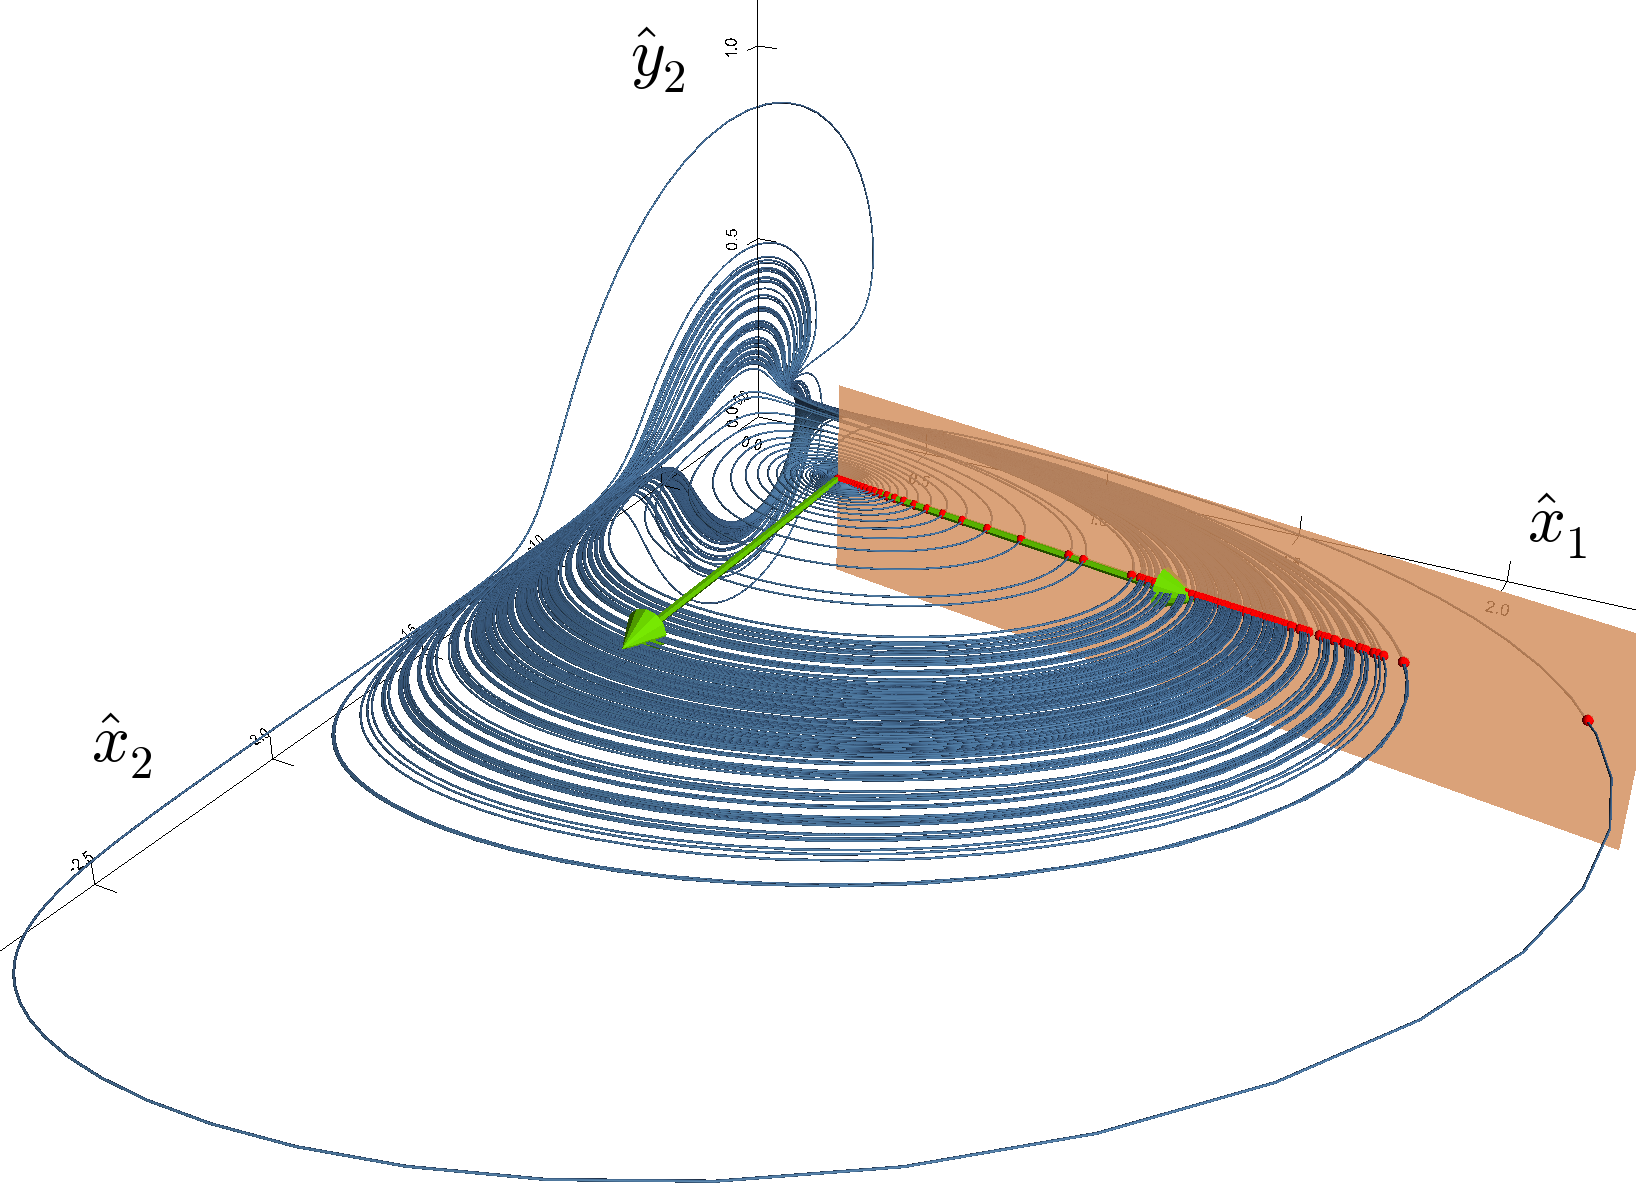
\includegraphics[width=0.45\textwidth]{BBpsecthd}
%\caption{
%Symmetry reduced flow within the slice hyperplane (blue). Green arrows show 
%the real and imaginary part of the unstable stability eigenvector $v_u$ of \REQV{}{1}. Poincar\'e section which includes $Re v_u$ is visualized as a transparent 
%plane, and intersections of the flow with the Poincar\'e section are marked with
%red.}
%\label{fig:BBpsecthd}
%\end{figure}

\begin{figure}
\centering
  (a) 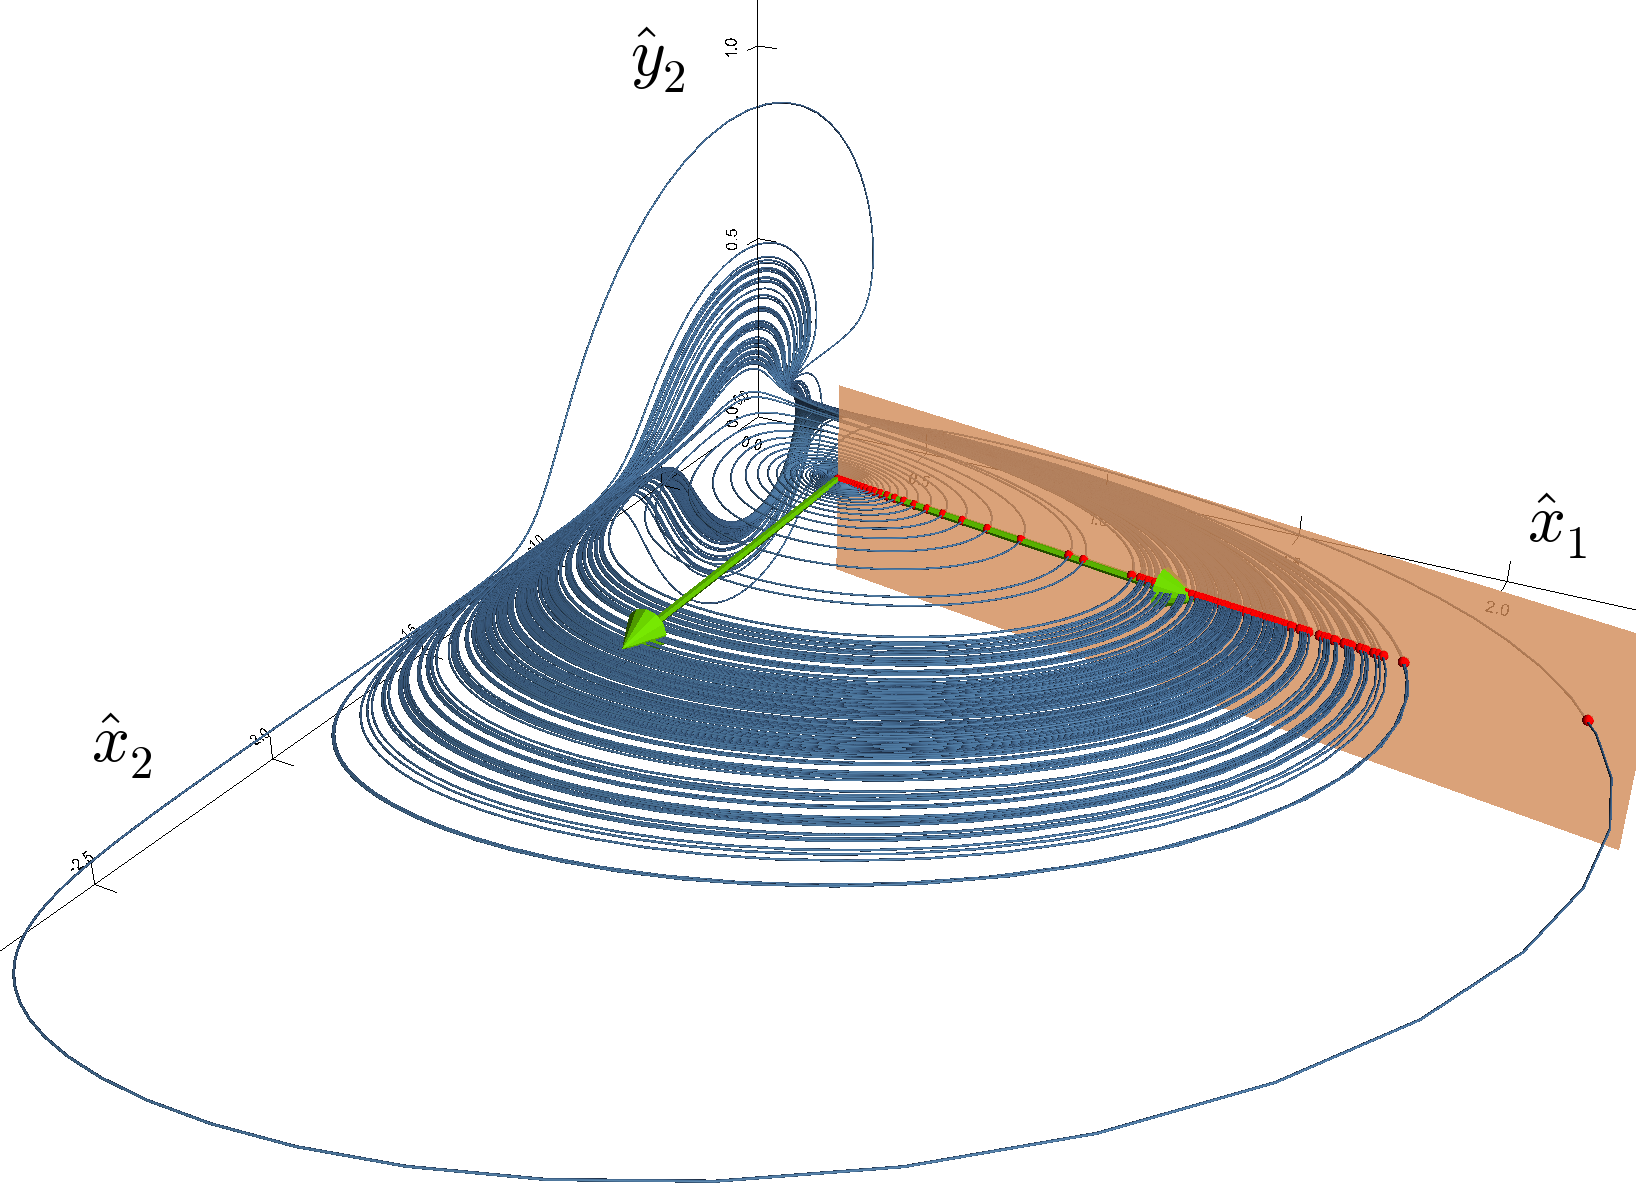
\includegraphics[width=0.45\textwidth]{BBpsecthd} \\
  (b) 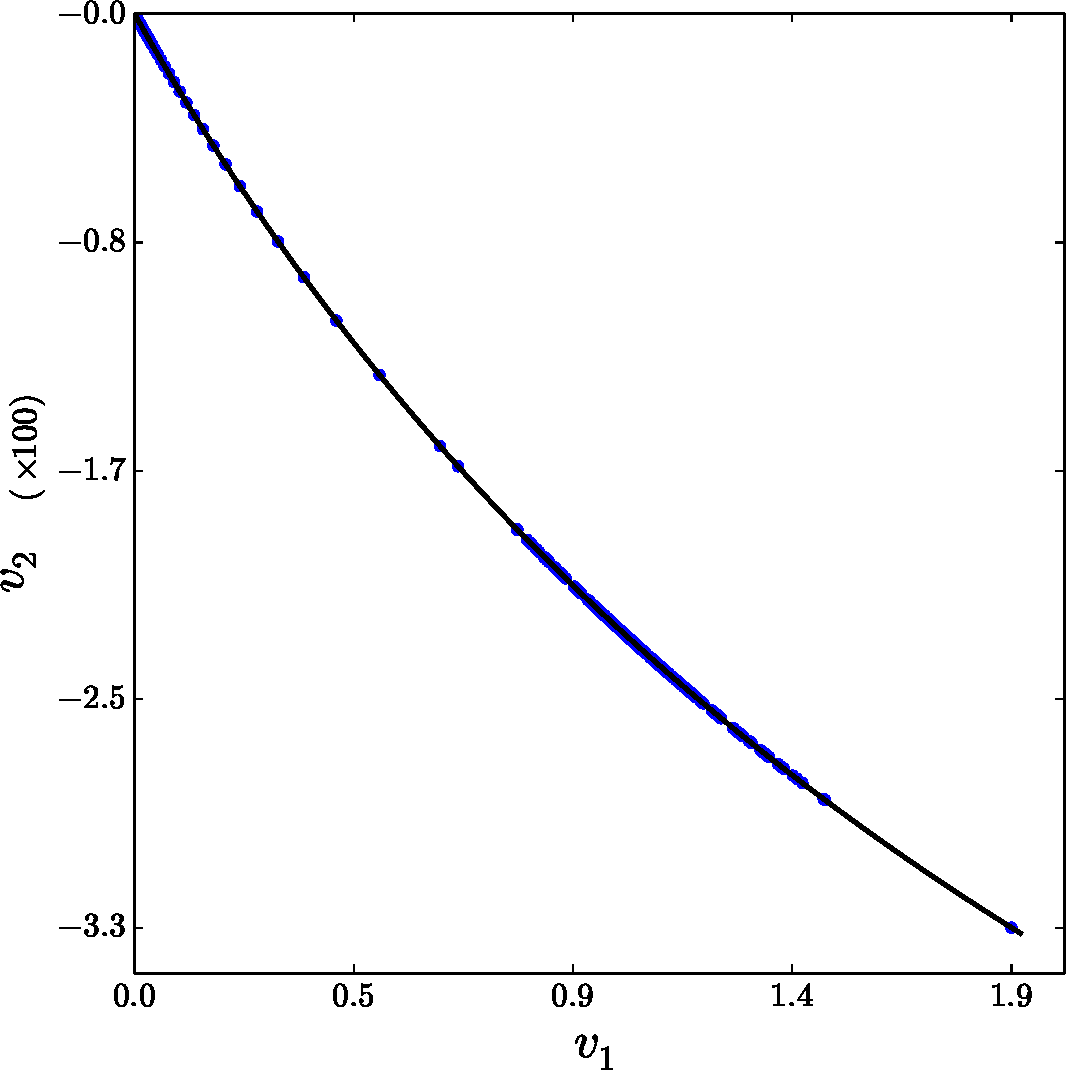
\includegraphics[width=0.20\textwidth]{BBpsectonslice}
  (c) 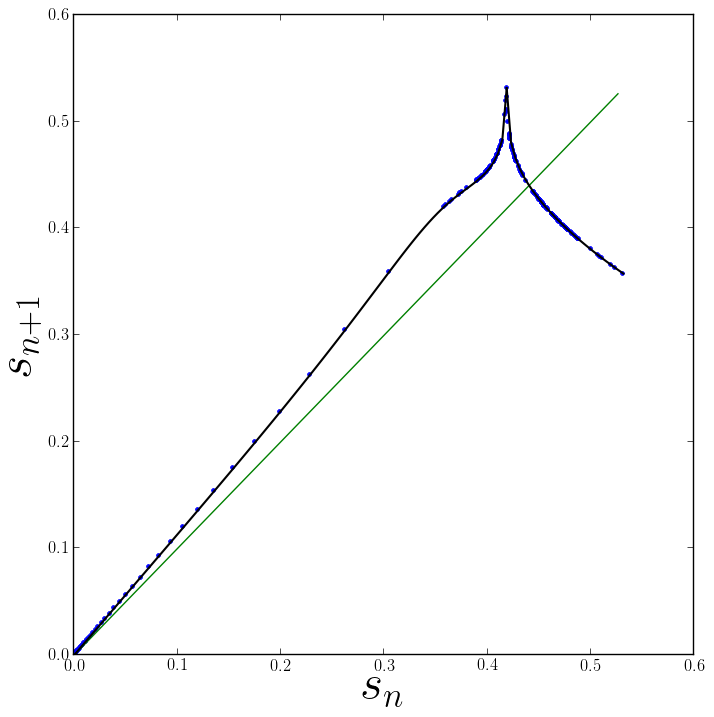
\includegraphics[width=0.20\textwidth]{BBretmaponslice} \\
  (d) 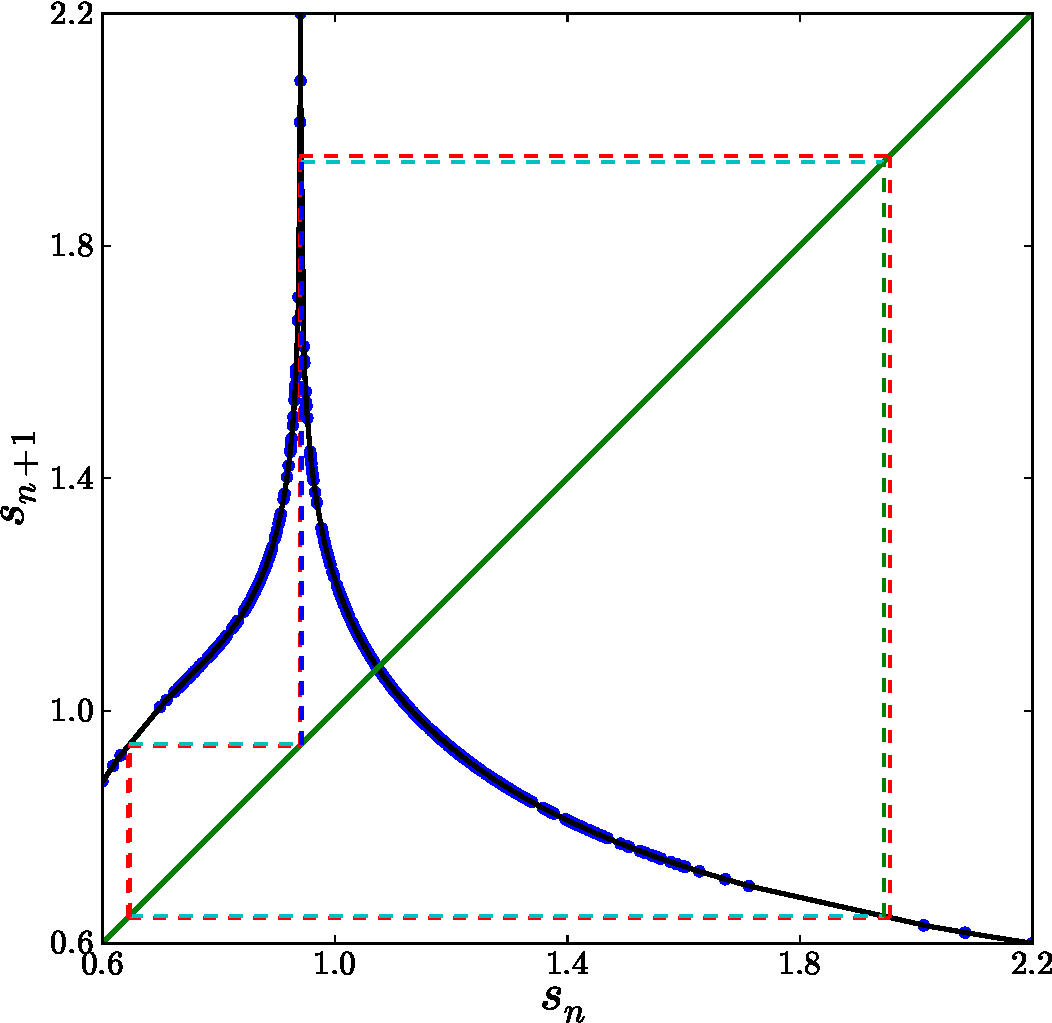
\includegraphics[width=0.45\textwidth]{BBretmaponsliceZoom}
\caption{(a)Symmetry reduced flow within the slice hyperplane (blue). 
			Green arrows show the real and imaginary part of the unstable stability 
			eigenvector $v_u$ of \REQV{}{1}. Poincar\'e section which includes 
			$Re[v_u]$ is visualized as a transparent plane, and intersections 
			of the flow with the Poincar\'e section are marked with red. 
		 (b)The Poincar\'e section which includes the \REQV{}{1} and $v_u$ projected
			on to the basis within the plane shown in (a). Note that 
		  	the vertical axis is magnified by $100$. 
		 (c)The Poincar\'e return map of arclengths along the 
		    Poincar\'e section in (b).
		 (d)Same return map without the transient points close to the \REQV{}{1}.
		 	Dashed lines show the cycle \cycle{010}.}
\label{fig:psectandretmap}
\end{figure}

%\begin{figure}%[H]
%\centering
 %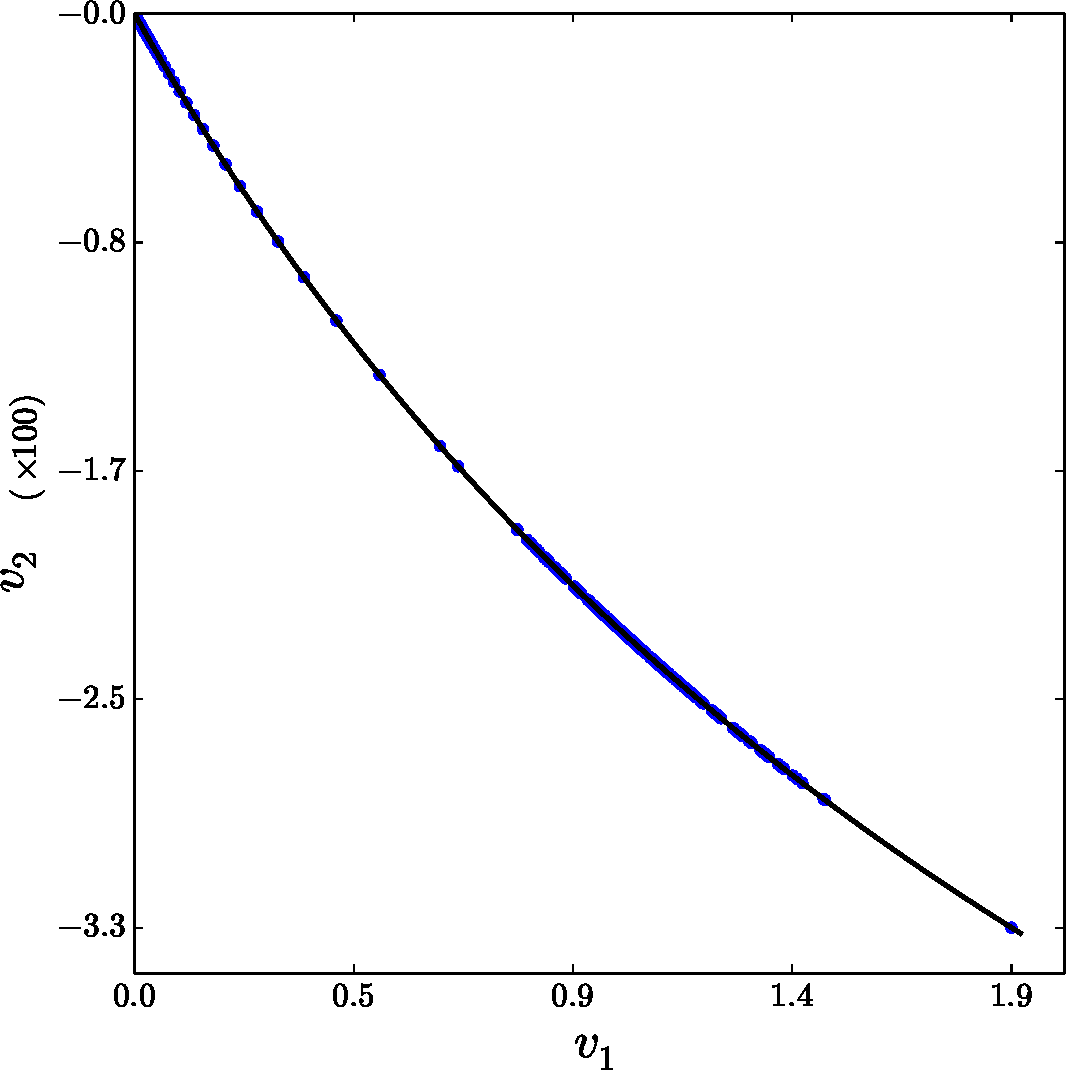
\includegraphics[width=0.45\textwidth]{BBpsectonslice}
%\caption{The Poincar\'e section involving the \reqv\ and its unstable direction.
		  %See \reffig{fig:BBpsecthd} for its 3D visualization.}
%\label{fig:BBpsectonslice}
%\end{figure}

%\begin{figure}%[H]
%\centering
 %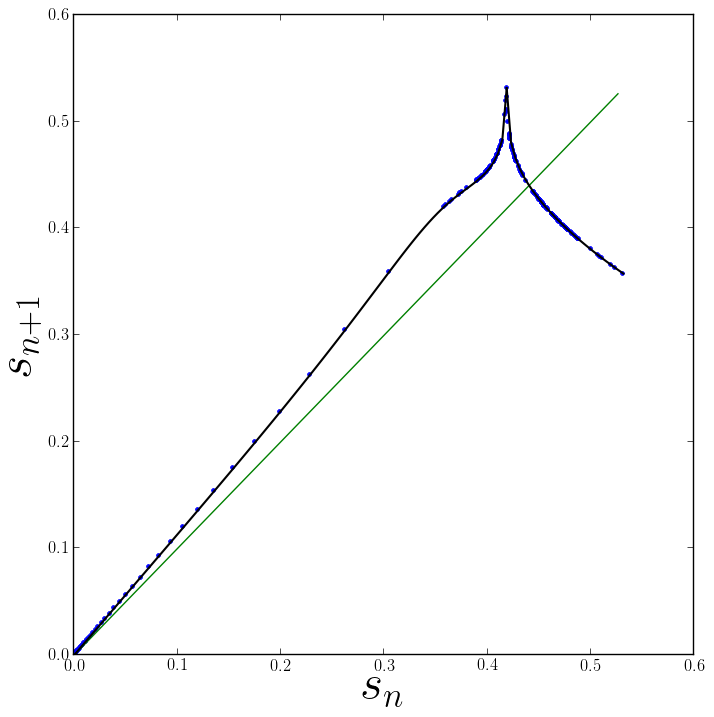
\includegraphics[width=0.45\textwidth]{BBretmaponslice}
%\caption{Poincar\'e return map of arclengths along the Poincar\'e section
		%shown in \reffig{fig:BBpsectonslice}.}
%\label{fig:BBretmaponslice}
%\end{figure}

\begin{figure}%[H]
  \begin{center}
  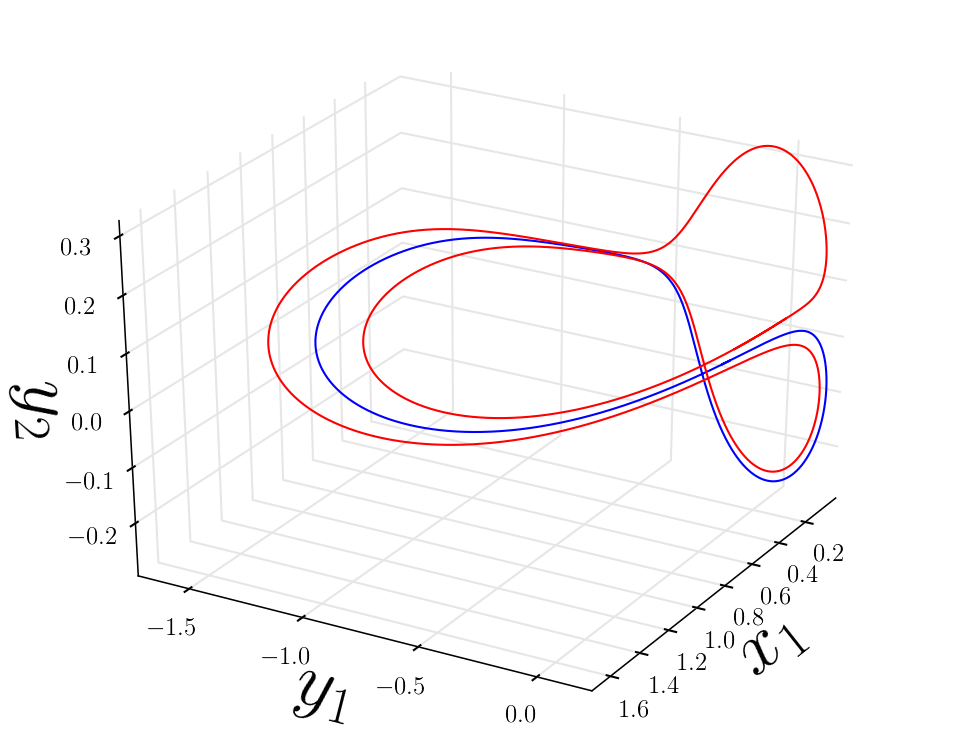
\includegraphics[width=0.45\textwidth]{BBrpo}
  \end{center}
  \caption{
	\Rpo s \cycle{1} and \cycle{01} embedded in the strange attractor
    of \reffig{fig:Set1}\,(d).
    }
  \label{fig:BBrpo1-01}
\end{figure}

\rpo s and their binary itineraries, the two shortest cycles
\cycle{1} and \cycle{01} are plotted in
\reffig{fig:BBrpo1-01}.
